\chapter{Implementasi}

\section{Deskripsi Persoalan dan Pemahaman Data}
Sebuah penginapan ingin memperkirakan pemesanan yang akan dibatalkan agar perencanaan kamar, overbooking, dan kebijakan pembatalan lebih akurat. Dataset Kaggle terdiri atas \texttt{train.csv} (27.373 baris, 17 fitur, dan target) dan \texttt{test.csv} (6.844 baris). Prediksi dinilai dengan Macro F1.

\begin{table}[H]
\centering
\caption{Fitur pada dataset}
\label{tab:fitur}
\begin{tabularx}{\textwidth}{>{\ttfamily\raggedright\arraybackslash}p{6.2cm}X}
\toprule
\normalfont\textbf{Fitur} & \textbf{Keterangan} \\
\midrule
num\_adults, num\_children & Jumlah tamu dewasa dan anak \\
weekend\_nights, weekday\_nights & Jumlah malam akhir pekan dan hari kerja \\
meal\_package & Paket makan (kategorikal) \\
needs\_parking & 1 jika membutuhkan parkir \\
room\_category & Kategori kamar Type A sampai G (kategorikal, tidak berurutan) \\
days\_before\_arrival & Selisih hari antara pemesanan dan kedatangan (lead time) \\
arrival\_year/month/day & Tanggal kedatangan \\
booking\_channel & Kanal pemesanan (kategorikal) \\
is\_returning\_guest & 1 jika tamu pernah menginap \\
prior\_cancellations, prior\_completed\_bookings & Riwayat pemesanan tamu \\
nightly\_rate\_idr & Harga rata-rata per malam (IDR) \\
special\_requests & Jumlah permintaan khusus \\
is\_canceled & Target (1 = batal) \\
\bottomrule
\end{tabularx}
\end{table}

Temuan utama dari eksplorasi data (bagian Data Understanding pada \texttt{src/main.ipynb}):
\begin{itemize}
  \item \textbf{Ketidakseimbangan kelas}: 67,2\% tidak batal dan 32,8\% batal (sekitar 2:1), tidak seimbang tetapi tidak ekstrem.
  \item \textbf{Missing value} pada delapan kolom, antara 3\% dan 11\% (Tabel~\ref{tab:missing}), dengan proporsi hampir sama di train dan test. Rasio batal baris kosong dan terisi hanya berbeda di bawah 2 poin persen, kecuali \texttt{special\_requests} (40,8\% jika kosong, 32,0\% jika terisi).
  \item \textbf{Duplikat dan nilai janggal}: 64 baris duplikat persis (fitur dan target), 106 pemesanan tanpa tamu dewasa, 64 pemesanan dengan total malam 0, 3 pemesanan dengan 9 atau 10 anak, dan 146 pemesanan berharga 0 di luar kanal Complimentary.
  \item \textbf{Skala fitur} sangat berbeda: \texttt{nightly\_rate\_idr} berada pada 0 sampai Rp9.165.000, sedangkan fitur biner hanya 0 sampai 1. Lead time sangat menceng ke kanan (median 58 hari, maksimum 448 hari).
  \item \textbf{Sinyal terkuat}: \texttt{days\_before\_arrival} (korelasi 0,44 dengan target, rasio batal naik dari 8,8\% pada lead time 0 sampai 5 hari menjadi 73,8\% di atas 192 hari), \texttt{special\_requests} ($-0{,}26$; 43,2\% batal tanpa permintaan khusus dan hampir tidak ada pembatalan pada 3 permintaan atau lebih), dan kanal pemesanan (Complimentary 0\%, Corporate 11,5\%, Online Travel Agent 36,4\%).
  \item \textbf{Pola musiman}: rasio batal terendah pada Januari (2,6\%) dan Desember (12,1\%), tertinggi pada Juli (44,8\%). Korelasi linear \texttt{arrival\_month} hampir nol ($-0{,}016$) karena polanya naik lalu turun, sehingga perlu encoding melingkar.
\end{itemize}

\begin{table}[H]
\centering
\caption{Persentase missing value pada train dan test}
\label{tab:missing}
\begin{tabular}{lrr}
\toprule
Kolom & Train (\%) & Test (\%) \\
\midrule
num\_children & 11,09 & 10,91 \\
special\_requests & 9,13 & 8,66 \\
nightly\_rate\_idr & 7,45 & 7,89 \\
meal\_package & 6,43 & 6,46 \\
days\_before\_arrival & 4,10 & 4,24 \\
needs\_parking & 3,95 & 3,61 \\
room\_category & 3,66 & 3,54 \\
num\_adults & 2,96 & 2,63 \\
\bottomrule
\end{tabular}
\end{table}

\begin{figure}[H]
\centering
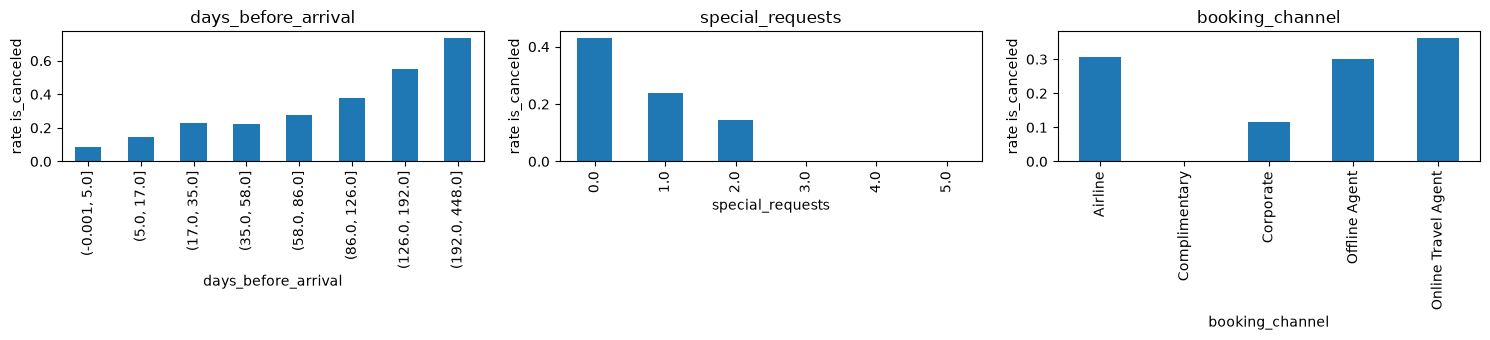
\includegraphics[width=\textwidth]{eda_target_rate.png}
\caption{Rasio batal per lead time, jumlah permintaan khusus, dan kanal pemesanan}
\label{fig:eda_rate}
\end{figure}

\begin{figure}[H]
\centering
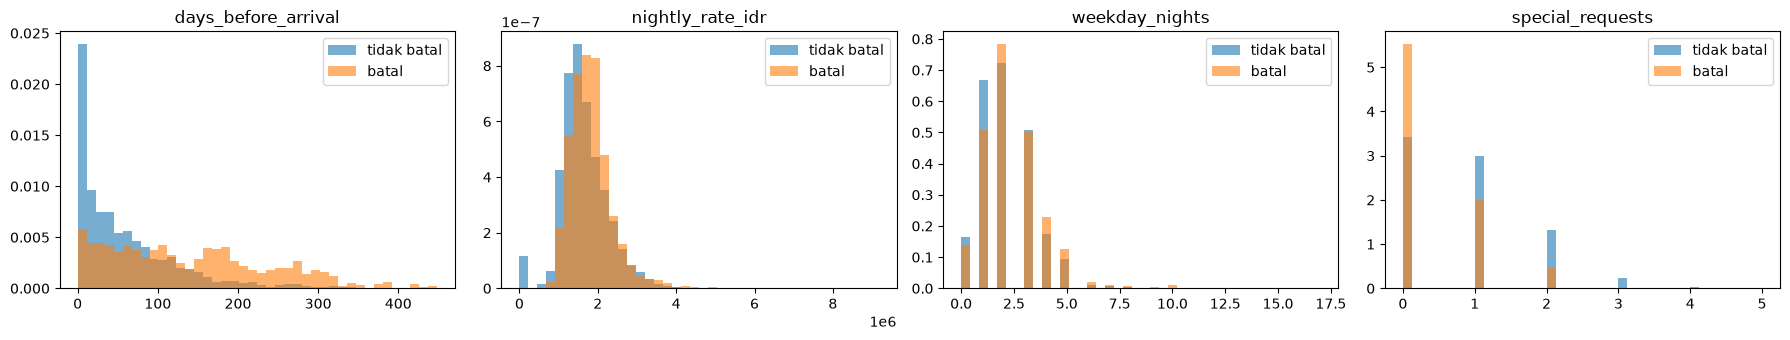
\includegraphics[width=\textwidth]{eda_histogram.png}
\caption{Distribusi fitur numerik per kelas (density)}
\label{fig:eda_hist}
\end{figure}

\begin{figure}[H]
\centering
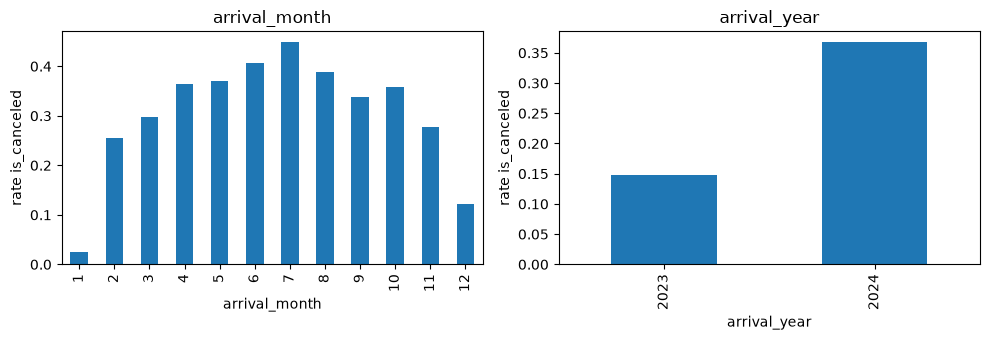
\includegraphics[width=0.8\textwidth]{eda_musim.png}
\caption{Rasio batal per bulan dan tahun kedatangan}
\label{fig:eda_musim}
\end{figure}

\begin{figure}[H]
\centering
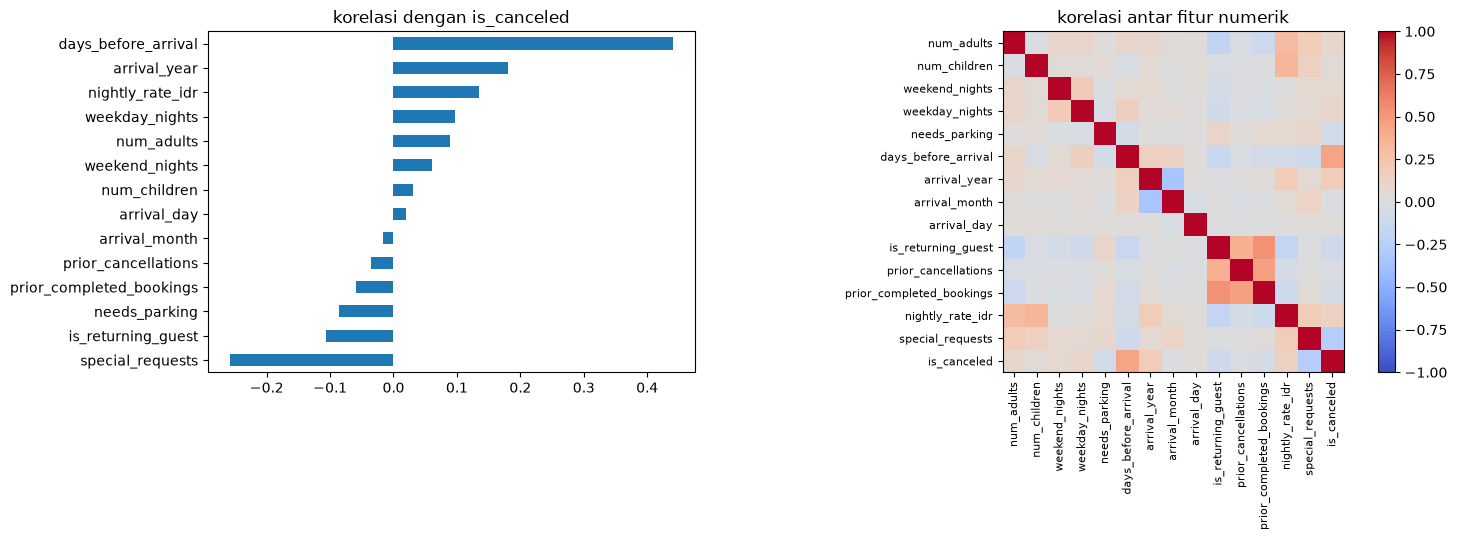
\includegraphics[width=\textwidth]{eda_korelasi.png}
\caption{Korelasi fitur numerik dengan target (kiri) dan antarfitur (kanan)}
\label{fig:eda_korelasi}
\end{figure}

\paragraph{Booking kembar dan noise.} Data ini diberi noise oleh penyelenggara. Untuk melihat kolom mana yang diberi noise, dicari pasangan pemesanan yang identik di semua kolom kecuali lead time dan tanggal datang. Dari 176 pasangan yang berdekatan, 93,2\% memiliki label yang sama. Tanggal datang hampir selalu sama (91,5\% berbeda paling banyak 1 hari, simpangan baku 1,98 hari), sedangkan lead time menyebar (hanya 25\% berbeda paling banyak 1 hari, simpangan baku 4,78 hari). Temuan ini menjadi dasar vote booking kembar pada model KNN final (Bagian~\ref{sec:knn}).

\begin{figure}[H]
\centering
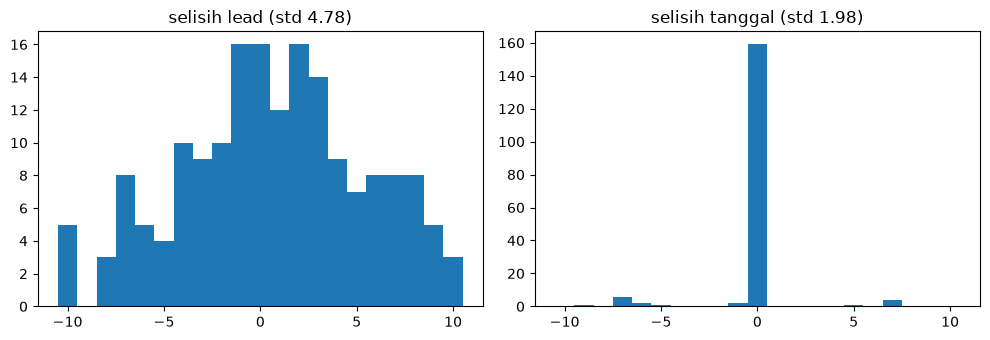
\includegraphics[width=0.8\textwidth]{eda_kembar.png}
\caption{Selisih lead time dan tanggal datang pada pasangan booking identik}
\label{fig:eda_kembar}
\end{figure}

\section{Struktur Program}
Seluruh kode from scratch (preprocessing, model, dan validasi) ditulis langsung di dalam notebook, tanpa modul Python terpisah. Format notebook mengikuti templat tugas.
\begin{itemize}
  \item \texttt{src/main.ipynb}: notebook final yang mereproduksi submission Kaggle. Berisi pemahaman data, preprocessing bersama, model KNN final, Decision Tree terbaik, perbandingan scikit-learn, save/load model, submission, error analysis, dan cost-sensitive classification.
  \item \texttt{src/experiments/<model>/}: notebook eksperimen tiap model (\texttt{knn}, \texttt{dtl}, \texttt{lr}, \texttt{svm}, \texttt{nb}). Satu notebook untuk satu eksperimen.
  \item \texttt{output/submissions/}: berkas submission; \texttt{output/models/}: model tersimpan (\texttt{.pkl}); \texttt{output/figures/}: gambar dan video untuk bonus.
\end{itemize}
Setiap model mengikuti antarmuka yang sama: \texttt{fit(X, y)}, \texttt{predict\_proba(X)} yang mengembalikan probabilitas kelas 1, dan \texttt{predict(X, threshold)}. Setiap notebook mencetak md5 berkas submission di akhir untuk membuktikan bahwa hasilnya reproducible.

\section{Data Cleaning dan Preprocessing}

\subsection{Preprocessing bersama}
Preprocessing bersama dipakai oleh KNN final dan Logistic Regression (notebook \texttt{lr\_main\_*}). Setiap langkah ditulis sebagai fungsi kecil yang menerima list \texttt{frames}, mengambil statistik dari \texttt{frames[0]} (data fit), lalu menerapkannya ke semua frame. Fungsi \texttt{prepare} menggabungkan semua langkah dengan urutan yang benar.

\begin{table}[H]
\centering
\caption{Langkah preprocessing bersama beserta alasannya}
\label{tab:prep_bersama}
\begin{tabularx}{\textwidth}{>{\raggedright\arraybackslash}p{3.3cm}>{\raggedright\arraybackslash}p{4.7cm}X}
\toprule
Langkah & Transformasi & Alasan \\
\midrule
Dedupe & Buang 64 baris duplikat (fitur dan target) sebelum split & Duplikat bisa berada di fold latih dan validasi sekaligus sehingga skor terlalu optimis \\
Data error & \texttt{num\_adults = 0} menjadi missing & Pemesanan tanpa tamu dewasa tidak masuk akal \\
Outlier & Clipping ke persentil 0,5\% dan 99,5\% data fit & Nilai ekstrem tidak mendominasi jarak \\
Fitur turunan & \texttt{booking\_index} (tanggal booking) dan \texttt{month\_cos} (musim) & Lead time dan tanggal datang digabung, Desember dan Januari berdekatan \\
Imputasi & Median (numerik), modus (kategorikal) dari data fit & Lebih baik dari mean, modus, KNN imputation, group median, dan jarak yang mengabaikan missing \\
Scaling & Robust scaler $(x-\text{median})/\text{IQR}$ & Tidak terpengaruh outlier, lebih baik dari z-score, min-max, dan rank \\
Bobot fitur & Lead time dan special\_requests $\times2$, needs\_parking dan weekday\_nights $\times0{,}5$, num\_adults $\times0{,}25$ & Hasil coordinate search, menekankan fitur yang paling informatif \\
Encoding & One-hot dengan nilai 0,75 & Kategori tidak berurutan, nilai 0,75 agar beda kategori tidak terlalu dominan \\
\bottomrule
\end{tabularx}
\end{table}

Hasilnya 15 fitur atau 28 kolom (12 numerik dan 16 one-hot). Reduksi dimensi dilakukan dengan seleksi fitur (forward selection), bukan PCA, agar fitur tetap dapat dijelaskan dan diberi bobot sendiri-sendiri. Ketidakseimbangan kelas tidak ditangani dengan resampling, tetapi dengan memilih threshold yang memaksimalkan Macro F1.

\begin{lstlisting}[caption={Pipeline preprocessing bersama (\texttt{src/main.ipynb})}, label={lst:prepare}]
def prepare(fit_df, *dfs):
    frames = [df.copy() for df in (fit_df,) + dfs]
    mark_invalid(frames)                                  # num_adults = 0 -> NaN
    cap_outliers(frames, clip_col, CFG.CLIP_QUANTILE)     # persentil 0.5% dan 99.5%
    engineer(frames)                                      # booking_index, month_cos
    impute(frames, num_col, 'median')
    impute(frames, cat_col, 'most_frequent')
    scale(frames, num_col)                                # robust scaler
    weight(frames, CFG.FEATURE_WEIGHTS)
    columns = num_col + encode(frames, cat_col, CFG.ONEHOT_VALUE)
    return [frame[columns].to_numpy(np.float32) for frame in frames]

def cap_outliers(frames, columns, q=0.005):
    lower, upper = frames[0][columns].quantile(q), frames[0][columns].quantile(1 - q)
    same = lower >= upper
    lower, upper = lower.where(~same, -np.inf), upper.where(~same, np.inf)
    for frame in frames:
        frame[columns] = frame[columns].clip(lower, upper, axis=1)

def scale(frames, columns):
    fit = frames[0][columns].astype(float)
    center = fit.median()
    spread = fit.quantile(0.75) - fit.quantile(0.25)
    spread = spread.where(spread > 0, fit.std()).replace(0, 1)
    for frame in frames:
        frame[columns] = (frame[columns].astype(float) - center) / spread
\end{lstlisting}

\subsection{Preprocessing khusus model}
Setiap algoritma memiliki asumsi berbeda terhadap bentuk data, sehingga sebagian eksperimen memakai preprocessing sendiri (Tabel~\ref{tab:prep_model}).

\begin{table}[H]
\centering
\caption{Preprocessing khusus model beserta alasannya}
\label{tab:prep_model}
\begin{tabularx}{\textwidth}{>{\raggedright\arraybackslash}p{2.4cm}>{\raggedright\arraybackslash}p{5.6cm}X}
\toprule
Model & Transformasi & Alasan \\
\midrule
DTL & Dedupe, \texttt{num\_adults = 0} jadi missing, 7 fitur turunan, kategori langka ($<20$ baris) menjadi \texttt{Other}. NaN dan kategori teks dibiarkan, tanpa scaling & Pohon menangani missing dan kategori langsung. Split berbasis urutan nilai sehingga tidak terpengaruh skala \\
LR & Indikator missing, imputasi median, \texttt{log1p}, encoding siklik, one-hot, binning berbasis target, interaksi fitur & Model linear butuh representasi yang menangkap hubungan tidak linear dan interaksi \\
SVM & Imputasi, one-hot, standardisasi, ditambah fitur turunan & Kernel dihitung dari hasil kali dalam atau jarak sehingga sensitif terhadap skala \\
NB & Setiap fitur menjadi kode kategori; lead time dikelompokkan ke $\le30$, 30 sampai 90, dan $>90$ hari; tarif ke $\le1$ juta, 1 sampai 2 juta, dan $>2$ juta. Nilai kosong menjadi kategori sendiri & Categorical Naive Bayes membutuhkan nilai diskrit \\
\bottomrule
\end{tabularx}
\end{table}

Tujuh fitur turunan pada DTL adalah \texttt{total\_nights}, \texttt{total\_guests}, \texttt{is\_free} (harga 0), \texttt{rate\_per\_guest}, \texttt{arrival\_weekday}, \texttt{arrival\_dayofyear}, dan \texttt{arrival\_index} (hari sejak 1 Januari 2023).

\begin{lstlisting}[caption={Preprocessing DTL (\texttt{src/experiments/dtl/})}, label={lst:prepare_tree}]
def group_rare(frames, columns, min_count=20):
    for column in columns:
        counts = frames[0][column].value_counts()
        keep = sorted(counts[counts >= min_count].index)
        for frame in frames:
            known = frame[column].isin(keep) | frame[column].isna()
            frame.loc[~known, column] = 'Other'

def prepare_tree(fit_df, *dfs):
    frames = [df.copy() for df in (fit_df,) + dfs]
    mark_invalid(frames)
    add_features(frames)
    frames = [f.drop(columns=[c for c in [ID, TARGET] if c in f.columns]) for f in frames]
    group_rare(frames, cat_col, CFG.RARE_MIN_COUNT)
    return frames          # NaN dan kategori teks dibiarkan untuk pohon
\end{lstlisting}

\section{Skema Validasi}
Semua preprocessing di-fit ulang di setiap fold hanya dengan data latih fold tersebut. Threshold dipilih dari grid 0,20 sampai 0,80 dengan langkah 0,01 berdasarkan Macro F1 OOF.
\begin{itemize}
  \item \textbf{Notebook final}: holdout 20\% stratified (seed 5) untuk membandingkan model, dan 5-fold OOF untuk skor akhir.
  \item \textbf{Eksperimen}: stratified 5-fold manual dengan seed 42. Setiap perubahan dicek ulang pada beberapa seed fold lain (seed 1 sampai 5 untuk DTL, seed 4, 5, dan 42 untuk KNN) agar kenaikan tidak hanya kebetulan dari satu pembagian data.
\end{itemize}
Model final dilatih ulang pada seluruh data latih, disimpan dengan \texttt{pickle}, lalu dimuat ulang untuk membuat submission.

\section{K-Nearest Neighbors}
\label{sec:knn}
Kelas \texttt{KNN} hanya memakai NumPy. Jarak Minkowski dijumlah per kolom dalam float32 agar memori cukup, lalu $k$ tetangga terdekat dipilih dengan \texttt{argpartition} dan diurutkan secara stabil. Model final memakai $k=17$, $p=1{,}5$, dan bobot vote $1/(d^2+10^{-6})$.

\begin{lstlisting}[caption={Kelas KNN (\texttt{src/main.ipynb})}, label={lst:knn}]
class KNN:
    def __init__(self, k=5, p=2.0, batch=1024):
        self.k, self.p, self.batch = k, p, batch

    def fit(self, X, y):
        self.X, self.y = X, np.asarray(y).astype(int)
        return self

    def kneighbors(self, Q):
        dists, ids = [], []
        for start in range(0, len(Q), self.batch):
            q = Q[start:start + self.batch]
            D = np.zeros((len(q), len(self.X)), np.float32)
            for j in range(self.X.shape[1]):
                D += np.abs(q[:, j, None] - self.X[None, :, j]) ** self.p
            idx = np.argpartition(D, self.k - 1, axis=1)[:, :self.k]
            d = np.take_along_axis(D, idx, 1)
            order = np.argsort(d, axis=1, kind='stable')
            ids.append(np.take_along_axis(idx, order, 1))
            dists.append(np.take_along_axis(d, order, 1) ** (1 / self.p))
        return np.vstack(dists), np.vstack(ids)

    def predict_proba(self, Q):
        d, idx = self.kneighbors(Q)
        w = 1 / (d ** 2 + 1e-6)
        return (w * self.y[idx]).sum(1) / w.sum(1)
\end{lstlisting}

\paragraph{Vote booking kembar.} Berdasarkan temuan noise pada lead time, KNN final digabung dengan vote dari \emph{booking kembar}: baris latih dengan kolom \texttt{twin\_key} (jumlah malam, kanal, status tamu, riwayat pemesanan) sama persis, kolom \texttt{twin\_soft} (jumlah tamu, parkir, paket makan, kamar, permintaan khusus) sama atau kosong, selisih lead time paling banyak 10 hari, selisih tanggal datang paling banyak 2 hari, dan selisih harga paling banyak 6\%. Jika ada minimal 2 kembar, probabilitas akhir adalah
\begin{equation}
  \hat{p} = 0{,}2\,\hat{p}_{\text{KNN}} + 0{,}8\,\frac{\text{jumlah kembar yang batal}}{\text{jumlah kembar}},
\end{equation}
dan label batal diberikan jika $\hat{p}\ge0{,}4845$. Toleransi lead time dibuat longgar dan toleransi tanggal datang dibuat ketat karena noise terutama ada pada lead time.

\begin{lstlisting}[caption={Vote booking kembar (diringkas)}, label={lst:twin}]
def twin_vote(A, B, y_B, lead, day, price):
    groups_b = B.groupby(twin_key, dropna=False).indices
    for key, ia in A.groupby(twin_key, dropna=False).indices.items():
        ib = groups_b.get(key)                 # kolom kunci harus sama persis
        if ib is None:
            continue
        a, b = A.iloc[ia], B.iloc[ib]
        ok = np.ones((len(ia), len(ib)), bool)
        for c in twin_soft:                    # sama, atau salah satunya kosong
            x, z = a[c].to_numpy()[:, None], b[c].to_numpy()[None, :]
            ok &= (x == z) | pd.isna(x) | pd.isna(z)
        ok &= abs_diff(a, b, 'days_before_arrival') <= lead
        ok &= date_diff(a, b) <= day
        ok &= rel_diff(a, b, 'nightly_rate_idr') <= price
        n = ok.sum(1)
        share[ia] = (ok * y_B[ib][None, :]).sum(1) / np.maximum(n, 1)
        count[ia] = n
    return share, count
\end{lstlisting}

\section{Decision Tree Learning (C4.5)}
Kelas \texttt{DecisionTree} mengimplementasikan pohon biner dengan pilihan criterion gini, entropy, atau gain ratio. Model terbaik memakai \textbf{gain ratio (C4.5)} dengan split biner. Implementasi ini menangani tiga jenis data yang diminta spesifikasi secara langsung:
\begin{itemize}
  \item \textbf{Numerik}: nilai diurutkan, lalu jumlah kumulatif label positif dipakai untuk menghitung impurity semua titik potong sekaligus. Threshold adalah titik tengah dua nilai berbeda yang berurutan.
  \item \textbf{Kategorikal}: kolom bertipe teks dikenali otomatis. Kategori diurutkan berdasarkan proporsi kelas positif, lalu dicari titik potong terbaik di antara peringkatnya, sehingga cukup mencoba $c-1$ titik potong.
  \item \textbf{Missing value}: split dicari dari baris yang terisi. Kedua kemungkinan (baris kosong ke kiri atau ke kanan) dievaluasi, dan arah dengan impurity terkecil disimpan sebagai arah default untuk prediksi. Kategori yang tidak dikenal saat prediksi juga mengikuti arah ini.
\end{itemize}
Sesuai C4.5, gain ratio hanya dihitung untuk split yang information gain-nya minimal sebesar rata-rata gain, agar split dengan split information sangat kecil tidak terpilih.

\begin{lstlisting}[caption={Pemilihan split dengan gain ratio (diringkas)}, label={lst:gainratio}]
if self.criterion == 'gain_ratio':
    # C4.5: gain ratio hanya untuk split point dengan gain >= rata-rata gain
    ok = gain > 1e-12
    if not ok.any():
        continue
    ok &= gain >= gain[ok].mean() - 1e-12
    split_info = _impurity(nl, np.full_like(nl, split_total), 'entropy')
    ratio = np.where(ok, gain / np.maximum(split_info, 1e-12), -np.inf)
    i = int(np.argmax(ratio))
    candidates.append((float(ratio[i]), make_split(i, float(gain[i]))))
\end{lstlisting}

Pre-pruning dilakukan dengan \texttt{max\_depth}, \texttt{min\_samples\_leaf}, dan \texttt{min\_impurity\_decrease} (minimum gain). Konfigurasi terbaik adalah gain ratio dengan \texttt{max\_depth} 30, \texttt{min\_samples\_leaf} 5, dan \texttt{min\_impurity\_decrease} $2\times10^{-4}$, dipilih dengan grid search yang memilih sel dengan rata-rata skor tetangga tertinggi agar tidak memilih puncak yang sempit.

\paragraph{Cost-complexity pruning.} Sebagai algoritma optimasi di luar materi kuliah (materi hanya membahas reduced-error pruning dan rule post-pruning), pohon dapat dipangkas setelah dibangun dengan cost-complexity pruning \cite{ref:breiman}:
\begin{equation}
  R_\alpha(T) = R(T) + \alpha\,|\tilde{T}|,
\end{equation}
dengan $R(T)$ jumlah impurity leaf yang dibobot proporsi sampel dan $|\tilde{T}|$ jumlah leaf. Sebuah node dijadikan leaf jika $R(\text{node})+\alpha \le R(\text{subtree})+\alpha\,|\tilde{T}_{\text{subtree}}|$.

\begin{lstlisting}[caption={Cost-complexity pruning}, label={lst:ccp}]
def cost_complexity_prune(self, alpha):
    crit = 'gini' if self.criterion == 'gini' else 'entropy'
    def visit(node):
        r_leaf = node.n_samples / self.n_total_ * float(_impurity(node.n_pos, node.n_samples, crit))
        if node.is_leaf:
            return r_leaf, 1
        r_left, n_left = visit(node.left)
        r_right, n_right = visit(node.right)
        r_sub, n_sub = r_left + r_right, n_left + n_right
        if r_leaf + alpha <= r_sub + alpha * n_sub:    # subtree tidak sebanding dengan leaf-nya
            node.left = node.right = None
            node.feature = None
            return r_leaf, 1
        return r_sub, n_sub
    visit(self.root_)
    return self
\end{lstlisting}

\section{Logistic Regression}
Kelas \texttt{LogisticRegression} meminimalkan log-loss dengan regularisasi L1, L2, atau Elastic Net. Bagian L2 masuk ke gradien, sedangkan bagian L1 yang tidak terdiferensiasi di nol ditangani dengan proximal step (soft-thresholding) sehingga bobot yang tidak penting benar-benar bernilai nol. Selain gradient descent biasa, tersedia solver \textbf{FISTA} \cite{ref:fista}: gradien dihitung di titik momentum Nesterov, ukuran langkah $1/L$ dihitung dari konstanta Lipschitz, dan momentum di-reset ketika arah langkah berbalik (adaptive restart).

\begin{lstlisting}[caption={Satu iterasi FISTA dengan proximal step L1 (diringkas)}, label={lst:fista}]
err = s * (sigmoid(zv) - y) / S
w_new = wv - lr * (X.T @ err + lam2 * wv)          # gradien log-loss + L2
b_new = bv - lr * float(err.sum())
if lam1 > 0:                                       # proximal step untuk L1
    w_new = xp.sign(w_new) * xp.maximum(xp.abs(w_new) - lr * lam1, 0.0)
if self.solver == 'fista':
    if float((wv - w_new) @ (w_new - w)) + (bv - b_new) * (b_new - b) > 0:
        t = 1.0                                    # adaptive restart
    t_next = (1.0 + np.sqrt(1.0 + 4.0 * t * t)) / 2.0
    beta = (t - 1.0) / t_next
    t = t_next
wv = w_new + beta * (w_new - w)                    # titik momentum Nesterov
bv = b_new + beta * (b_new - b)
\end{lstlisting}

Tuning dilakukan dalam empat tahap preprocessing khusus model linear (\texttt{lr\_fe}, \texttt{lr\_target\_bins}, \texttt{lr\_l1\_onehot}, \texttt{lr\_cross\_bins}), ditambah dua notebook yang memakai preprocessing bersama (\texttt{lr\_main\_prep} dan \texttt{lr\_main\_expand}).

\section{Support Vector Machine}
Kelas \texttt{SVM} menyelesaikan bentuk dual untuk kernel linear, polynomial, dan Gaussian. Subproblem QP diselesaikan dengan SLSQP dalam blok working set berisi paling banyak 64 variabel alpha, sehingga matriks kernel penuh tidak perlu disimpan. Fungsi keputusan $f(x)=\sum_{i\in SV}\alpha_i y_i K(x_i,x)+b$ dikalibrasi menjadi probabilitas dengan Platt scaling menggunakan holdout internal 20\%. Hyperparameter $C$ dan $\gamma$ dicari dengan \textbf{Particle Swarm Optimization (PSO)} \cite{ref:pso,ref:pso_shi}: setiap partikel adalah kandidat $(\log_{10}C, \log_{10}g)$, dan posisinya diperbarui dengan
\begin{equation}
  v_i \leftarrow w v_i + c_1 r_1 (p_i - x_i) + c_2 r_2 (g^{*} - x_i), \qquad x_i \leftarrow x_i + v_i,
\end{equation}
dengan fitness berupa Macro F1 OOF. \todo{Akram: lengkapi detail implementasi dan hasil PSO dari notebook \texttt{svm.ipynb} terbaru.}

\section{Naive Bayes}
Kelas \texttt{NaiveBayes} mengimplementasikan Categorical Naive Bayes dengan Laplace smoothing ($\alpha=1$) pada kode kategori. Prior dan likelihood disimpan dalam bentuk logaritma, lalu probabilitas dinormalisasi dengan log-sum-exp agar stabil. Dua eksperimen dijalankan: dua fitur (\texttt{booking\_channel} dan \texttt{special\_requests}) dan semua 17 fitur asli.

\section{Pembanding scikit-learn}
Setiap model from scratch dibandingkan dengan scikit-learn \cite{ref:sklearn} memakai data, preprocessing, dan aturan threshold yang sama.
\begin{itemize}
  \item \textbf{KNN}: \texttt{KNeighborsClassifier(algorithm='brute')} dengan $k$, $p$, dan bobot jarak yang sama.
  \item \textbf{DTL}: \texttt{DecisionTreeClassifier} dengan parameter yang sama (entropy, karena scikit-learn tidak memiliki gain ratio), serta tiga varian yang diminta spesifikasi:
  \begin{itemize}
    \item ID3: \texttt{criterion='entropy'},
    \item C4.5: \texttt{criterion='entropy'} ditambah \texttt{ccp\_alpha},
    \item CART: \texttt{criterion='gini'}.
  \end{itemize}
  Karena scikit-learn tidak menerima teks dan NaN, kategori di-one-hot dan missing diisi median.
  \item \textbf{LR}: \texttt{LogisticRegression} (lbfgs untuk L2, saga untuk L1) pada matriks fitur yang sama.
  \item \textbf{SVM}: \texttt{SVC} dengan kernel dan parameter yang sama. Probabilitasnya dikalibrasi dengan \texttt{CalibratedClassifier\-CV}.
  \item \textbf{Naive Bayes}: \texttt{CategoricalNB(alpha=1)} pada kode kategori yang sama.
\end{itemize}
